\documentclass{article}
%packages
\usepackage{graphicx}
\usepackage[utf8]{inputenc}
\usepackage[T1]{fontenc}
\usepackage[frenchb]{babel}
\usepackage[a4paper]{geometry}
\usepackage{minted}

\begin{document}
%title
\begin{titlepage}
	\vspace{-20px}
	\begin{tabular}{l}
		\textsc{Blin} S\'ebastien\\
		\textsc{Collin} Pierre-Henri
	\end{tabular}
	\hfill \vspace{10px}
\includegraphics[scale=0.1]{esir.png}\\
	\vfill
	\begin{center}
		\Huge{\'Ecole sup\'erieure d'ing\'enieurs de Rennes}\\
		\vspace{1cm}
		\LARGE{1\`ere Ann\'ee}\\
		\large{Parcours Informatique}\\
		\vspace{0.5cm}\hrule\vspace{0.5cm}
		\LARGE{\textbf{Algorithmie et complexité}}\\
		\Large{Compte-Rendu TP1}
		\vspace{0.5cm}\hrule
		\vfill
		\vfill
	\end{center}
	\begin{flushleft}
		\Large{Sous l'encadrement de~:}\\
		\vspace{0.2cm}
		\large{{Ridoux} Olivier}\\
		\large{{Maurel} Pierre}
	\end{flushleft}
	\vfill
\end{titlepage}


\section{Problème des N reines}
\subsection{Objectif}
Dans la seconde partie de ce TP, nous devions utiliser les ROBDD pour pouvoir résoudre un problème. Le problème consiste à trouver une combinaison de cases où placer N dames sur un plateau de taille NxN pour ne pas qu'elles puissent se menacer mutuellement. Donc qu'il y en ait une par colonne, une par ligne, et pas 2 sur la même diagonale.\\
La solution consiste donc à modéliser une équation booléenne modélisant les conditions en prenant chaque case comme une variable.
\subsection{Moyens mis en \oe uvre}
L'expression finale est un ET logique entre 3 sous équations.\\
La première sous-équation décrit le fait qu'il y ait une dame par ligne.
\begin{minted}{java}
for(int i = 0; i < n; ++i)
{
	Expression temp2 = new Constante(false);
	for(int k = 0; k < n; ++k)
	{
		Expression temp = new Constante(true);
		for(int j = 0; j < n; ++j)
		{
			if(j != k)
				temp = new Et(new Non(new Atome("x"+ i + j)), temp);
			else
				temp = new Et(new Atome("x"+ i + j), temp);
		}
		temp2 = new Ou(temp2, temp);
	}
	expDame = new Et(expDame, temp2);
}
\end{minted}
Ce qui peut se traduire par $x_{ij}\Rightarrow \wedge_{1\geq l\geq N, l\neq j}\neg x_{il}$. Même si dans notre code, nous le modélisons à l'aide de Et et de Ou logique.\\
Pour les colonnes, c'est à peut prêt la même méthode, il suffit d'échanger 2 boucles.
\begin{minted}{java}
for(int j = 0; j < n; ++j)
{
	Expression temp2 = new Constante(false);
	for(int k = 0; k < n; ++k)
	{
		Expression temp = new Constante(true);
		for(int i = 0; i < n; ++i)
		{
			if(i != k)
				temp = new Et(new Non(new Atome("x"+ i + j)), temp);
			else
				temp = new Et(new Atome("x"+ i + j), temp);
		}
		temp2 = new Ou(temp2, temp);
	}
	expDame = new Et(expDame, temp2);
}
\end{minted}
Le traitement des diagonales est un peu différent. Ici, il faut considérer des droites et prendre seulement les cases dans le plateau. L'équation nous donne : $x_{ij}\Rightarrow \wedge_{1\geq k\geq N, 1\geq j+k-i\geq N, k\neq i}\neg x_{k,j+k-i}$ dans un sens, $x_{ij}\Rightarrow \wedge_{1\geq k\geq N, 1\geq j+i-k\geq N, k\neq i}\neg x_{k,j+i-k}$ pour l'autre sens.
\begin{minted}{java}
//Traitement des diagonales 
for(int i = 0; i < n; ++i)
{
	Expression temp2 = new Constante(false);
	for(int j = 0; j < n; ++j)
	{
		Expression temp = new Constante(true);
		for(int k = 0; k < n; ++k)
		{
			int v = j+k-i;
			int w = j+i-k;
			if(i != k && v < n && v >= 0)
				temp = new Et(new Non(new Atome("x" + k + v)), temp);
			else if(i!=k && w < n && w >= 0)
				temp = new Et(new Non(new Atome("x" + k + w)), temp);
			else
				temp = new Et(new Atome("x" + i + j), temp);
		}
		temp2 = new Ou(temp2, temp);
	}
	expDame = new Et(expDame, temp2);
}
\end{minted}
Enfin, pour la partie de l'affichage, il suffit de trouver une solution (première partie de la fonction) et de stocker les cases où les dames sont présentes à true. Puis on dessine avec la seconde partie de la fonction.
\begin{minted}{java}
//Affiche le tableau solution pour le probleme des dames
public void reines_affiche_sat(int n)
{
	//Le tableau contenant true pour les cases possedant une dame
	boolean[] solution = new boolean[n*n];
	Iterator<Noeud_ROBDD> it = R.iterator();
	int toSearch = 1;
	while(it.hasNext())
	{
		Noeud_ROBDD node = it.next();
		if(node.getIdFilsDroit() == toSearch)
		{
			toSearch = node.getId();
			try
			{
				//Pour savoir quelle variable correspond a quelle case
				Pattern p = Pattern.compile("x([0-9])([0-9])");
				Matcher m = p.matcher(node.getNom());
				m.matches();
				solution[Integer.parseInt(m.group(1))*n+
				Integer.parseInt(m.group(2))] = true;
			}
			catch (Exception e)
			{
			
			}
		}
		if(node.getIdFilsGauche() == toSearch)
			toSearch = node.getId();
	}
	
	/**Affichage**/
	for(int i = 0; i < n; ++i)
	{
		for(int j = 0; j < 3*n; ++j)
			System.out.print("_");
		System.out.print("\n");
		for(int j = 0; j < n; ++j)
			if(solution[i*n+j])
				System.out.print("|X|");
			else
				System.out.print("| |");
		System.out.print("\n");
	}
	for(int j = 0; j < 3*n; ++j)
		System.out.print("_");
	System.out.print("\n");
}
\end{minted}
\subsection{Résultats}
Pour un plateau de où N = :
\begin{itemize}
  \item 1 : le problème est SAT
  \item 2, 3 : NON SAT
  \item 4 : x13.x01.x20.x32.
  \item 5 : x02.x21.x40.x14.x33.
  \item 6 : x02.x21.x40.x15.x34.x53.
  \item 7 : x01.x40.x32.x24.x63.x16.x55.
  \item 8 : x06.x43.x30.x71.x22.x64.x15.x57.
\end{itemize}
Pour 8, la résolution commence à être longue, mais le ROBDD est conséquent.
\begin{figure}
	\begin{center}
		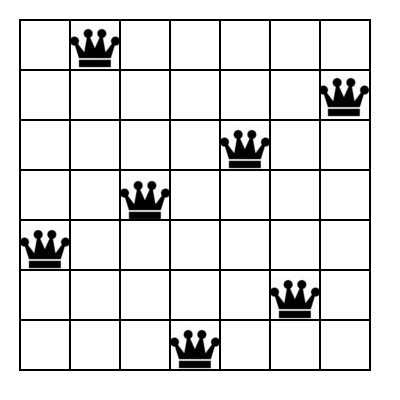
\includegraphics[scale=0.7]{sevenkingdom}\\
		Solution pour 7 reines
	\end{center}
\end{figure}
\section{Conclusion}
TODO : ROBDD bonne forme pour résoudre des problemes comme SAT
\end{document}

